\chapter{Charakterystyka ruchu pieszych}
\label{cha:charakterystykaRuchu}

\section{Points of intrest}
\label{sec:pointsOfInterest}
 Points
 
\section{Strefa prywatna}
\label{sec:strefaPryw}

Dla każdego pieszego definiuje się opisaną wcześniej strefę prywatna.
Im bliżej przeszkody lub innego agenta, tym pieszy czuje się mniej komfortowo i utrzymuje dystans od sąsiada zależny od konkretnej sytuacji. Strefa prywatna pomaga unikać kolizji w przypadkach nagłej zmiany prędkości przez innych uczestników ruchu.

\section{Czas relaksacji}
\label{sec:czasRelaksacji}

Piesi zmieniając kierunek swojej drogi potrzebują pewien (niewielki) czas na podjęcie decyzji. Z tego względu we wzorze został wprowadzony \textit{czas realaksacji}. Wartość przyjęta w symulacji to $0.5 sek$

\section{Czekający piesi}
\label{sec:czekajacyPiesi}

Czekający piesie są częstymi uczestnikami normalnego ruchu. Często zatrzymujemy się, aby porozmawiać przez telefon, zawiązać sznurowadła czy w oczekiwaniu na przyjazd windy. Czekający piesi mogą powodować korki \cite{6}. Modelowanie czekających pieszych ma dwa aspekty: reakcje  przechodzących obok pieszych na pozostającego w spoczynku oraz pozosrającego w spoczynku na poruszających się.

\section{Formowanie strug}
\label{sec:strugi}

\section{Unikanie Kolizji}
\label{sec:kolizje}

Podczas każdej zmiany położenia podczas symulacji należy sprawdzić czy po przejściu nie dojdzie do kolizji z innymi uczestnikami ruchu czy przeszkodami. Jeśli dojdzie do kolizji należy sprawdzić jakiego jest ona typu i dostosować do niej zachowanie. Do kolizji może dość w przypadku kiedy dwoje pieszych w następnym kroku mają przejść na to samo miejsce lub kiedy zamieniają się miejscami. Każda z kolizji wymaga podjęcia innych kroków, aby jej uniknąć. Po uniknięciu kolizji pieszy powinien powrócić do swojej pierwotnej ścieżki ruchu. Każdy z pieszych ma także pewien priorytet zależny od tego czy niepełnosprawny itp

Zgodnie z pracą \cite{Collision} możemy wyróżnić trzy typy kolizji:

\subsection{Kolizja czołowa}

Występuje w przypadku kiedy dwoje pieszych idą prosto na siebie. Na samym początku należy określić czy piesi kolidują ze sobą po lewej czy po prawej stronie (rzadko zdarza się ruch dokładnie na wprost siebie). Piesi preferują takie uniknięcie kolizji, jakie pozwoli im na jak najmniejsze odchylenie od ich, wyznaczonej wcześniej, trasy. Na bazie obserwacji możemy wyróżnić trzy możliwości uniknięcia takiej kolizji:

\begin{itemize}
\item zmianę kierunku ruchu
\item zmianę prędkości
\item zmianę zarówno kierunku jak i prędkości
\end{itemize}

Jeśli żadne z tych nie zdziała to pieszy zwyczajnie się zatrzyma. Pozwoli to na przejście innego pieszego, który ominie tego co stoi a ten co stoi pójdzie sobie potem dalej.


\begin{figure}
\centering
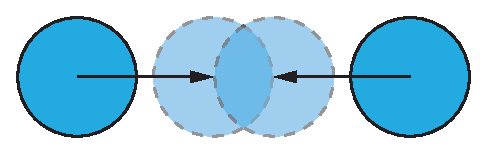
\includegraphics[width=0.4\textwidth]{kolizjaczolowa.eps}
\caption{Schemat kolizji czołowej, opracowanie własne}
\end{figure}

\subsection{Kolizja boczna}

Kolizja, której rozwiązanie jest podobne jak dla \textit{kolizji czołowej}.

\begin{figure}
\centering
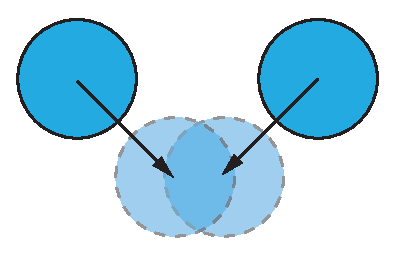
\includegraphics[width=0.4\textwidth]{kolizjaboczna.eps}
\caption{Schemat kolizji czołowej, opracowanie własne}
\end{figure}

\subsection{Kolizja tylna}

Ma miejsce kiedy jeden z kolidujących pieszych jest ze innym pieszym, ale ma wyższą prędkość ruchu, więc jaskoczy na niego. W tym przypadku są dwie drogi rozwiązania

\begin{itemize}
\item zwolnić do takiej samej prędkości jak pieszy z przodu i iść za nim
\item przyśpieszyć i wyprzedzić kolidującego pieszego z którejś ze stron
\end{itemize}

\begin{figure}
\centering
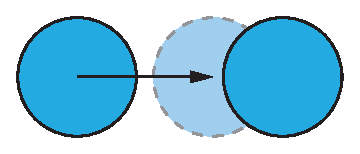
\includegraphics[width=0.4\textwidth]{kolizjatylna.eps}
\caption{Schemat kolizji czołowej, opracowanie własne}
\end{figure}
